% This is samplepaper.tex, a sample chapter demonstrating the
% LLNCS macro package for Springer Computer Science proceedings;
% Version 2.20 of 2017/10/04
%
\PassOptionsToPackage{prologue,table,xcdraw}{xcolor}
\documentclass[runningheads]{llncs}
\usepackage{times}

%\usepackage[prologue,table,xcdraw]{xcolor}
\usepackage{hyperref}
\renewcommand\UrlFont{\color{blue}\rmfamily}
\usepackage[title]{appendix}
%\usepackage{cite}
\usepackage{tablefootnote}
\usepackage{multirow}
\usepackage{amsmath}
\usepackage{siunitx}
%\usepackage{amssymb}
\usepackage{amsfonts}
\usepackage{algorithmic}
\usepackage{algorithm}
\usepackage{diagbox}
\usepackage{booktabs}
%% MAR: newlines in cells
\usepackage{makecell}
\usepackage{stackengine}
\renewcommand\theadalign{tl}
\renewcommand\theadfont{\bfseries}
\renewcommand\theadgape{\Gape[1pt]}
\renewcommand\cellgape{\Gape[1pt]}
%%%%%%%%%%%%%%%
\usepackage{textcomp}
\usepackage{xcolor}
\usepackage[numbers,sort&compress,sectionbib]{natbib}
%\usepackage[hyphens]{url}
\usepackage[nameinlink,capitalize]{cleveref}
\usepackage{hyperref}

\def\BibTeX{{\rm B\kern-.05em{\sc i\kern-.025em b}\kern-.08em
    T\kern-.1667em\lower.7ex\hbox{E}\kern-.125emX}}
    
% Image related packages
\usepackage{graphicx} %draft
\usepackage[export]{adjustbox}
\usepackage{subfig}
\usepackage{epstopdf}
\DeclareGraphicsExtensions{.pdf,.png,.eps,.jpg,.jpeg,.tif,.tiff,.ps}
\graphicspath{{images//}}

    
\usepackage{soul}
\usepackage{xspace}
\definecolor{navy}{rgb}{0.1, 0.1, 0.8}
\definecolor[named]{gray}{rgb}{0.4, 0.4, 0.4}
\definecolor[named]{olive}{rgb}{0.1, 0.5, 0.1}
\definecolor[named]{ruby}{rgb}{0.8, 0.1, 0.3}
\definecolor{darkpastelgreen}{rgb}{0.01, 0.75, 0.24}
\definecolor{celestialblue}{rgb}{0.29, 0.59, 0.82}
\definecolor{coral}{rgb}{1.0, 0.5, 0.31}
\definecolor{Goldenrod}{rgb}{0.8,0.8,0}

%%%%%%%% comments -- ENABLE (draft) %%%%%%%%%%%%%%
\usepackage[colorinlistoftodos,textsize=tiny]{todonotes}
\newcommand{\eat}[1]{}
\newcommand{\rev}[1]{{\color{olive}{#1}}}
\newcommand{\revA}[1]{{\color{navy}{#1}}}
\newcommand{\verify}[1]{{\color{red}{#1}}}
\newcommand{\verifyK}[1]{{\color{blue}{#1}}}
%\newcommand{\note}[1]{\todo[linecolor=red,backgroundcolor=red!25,bordercolor=red]{#1}}
\newcommand{\editnote}[2][1=]{\todo[linecolor=blue,backgroundcolor=blue!25,bordercolor=blue,#1]{#2}}
\newcommand{\mar}[1]{\todo[linecolor=navy,backgroundcolor=navy!25,bordercolor=navy]{\textbf{MAR:} #1}\xspace}
\newcommand{\cl}[1]{\todo[linecolor=darkpastelgreen,backgroundcolor=darkpastelgreen!25,bordercolor=darkpastelgreen]{\textbf{CL:} #1}\xspace}

\newcommand{\TODO}[2]{
\hl{ \textbf{#1}: #2}
}
\newcommand{\REV}[2]{
\todo[inline, color=blue!20]{{\bf #1}:~{#2}}
}

%%%%%%%% comments -- DISABLE (submission) %%%%%%%%%%%%%%%
% \newcommand{\eat}[1]{}
% \newcommand{\rev}[1]{{#1}}
% \newcommand{\rvx}[1]{{#1}}
% \newcommand{\revA}[1]{{#1}}
% \newcommand{\verify}[1]{#1}
% \newcommand{\verifyK}[1]{{#1}}
% \newcommand{\NOTE}[2]{}
% \newcommand{\TODO}[2]{}
% \newcommand{\nb}[1]{}
% \newcommand{\mar}[1]{}
% \newcommand{\cl}[1]{}


%% sqished lists
\newcommand{\squishlist}{
 \begin{list}{$\bullet$}
  { \setlength{\itemsep}{0pt}
     \setlength{\parsep}{3pt}
     \setlength{\topsep}{3pt}
     \setlength{\partopsep}{0pt}
     \setlength{\leftmargin}{1.5em}
     \setlength{\labelwidth}{1em}
     \setlength{\labelsep}{0.5em} } }

\newcommand{\squishlisttwo}{
 \begin{list}{$\bullet$}
  { \setlength{\itemsep}{0pt}
    \setlength{\parsep}{0pt}
    \setlength{\topsep}{0pt}
    \setlength{\partopsep}{0pt}
    \setlength{\leftmargin}{1.5em}
    \setlength{\labelwidth}{1.5em}
    \setlength{\labelsep}{0.5em} } }

\newcommand{\squishend}{
  \end{list}  }  
% Used for displaying a sample figure. If possible, figure files should
% be included in EPS format.
%
% If you use the hyperref package, please uncomment the following line
% to display URLs in blue roman font according to Springer's eBook style:
% \renewcommand\UrlFont{\color{blue}\rmfamily}


\begin{document}
\appendix

\noindent{\bf \huge Appendix}
\vspace{0.5cm}

This document is accompanying the submission \textit{Linking User Opinion Dynamics and Online Discussions}.
The information in this document complements the submission, and it is presented here for completeness reasons.
It is not required for understanding the main paper, nor for reproducing the results.

\section{Posting analysis and dataset profiling}

\begin{figure}[htbp]
	\centering
	\newcommand\myheightA{0.18} %% full size: 0.173
	\subfloat[]{
		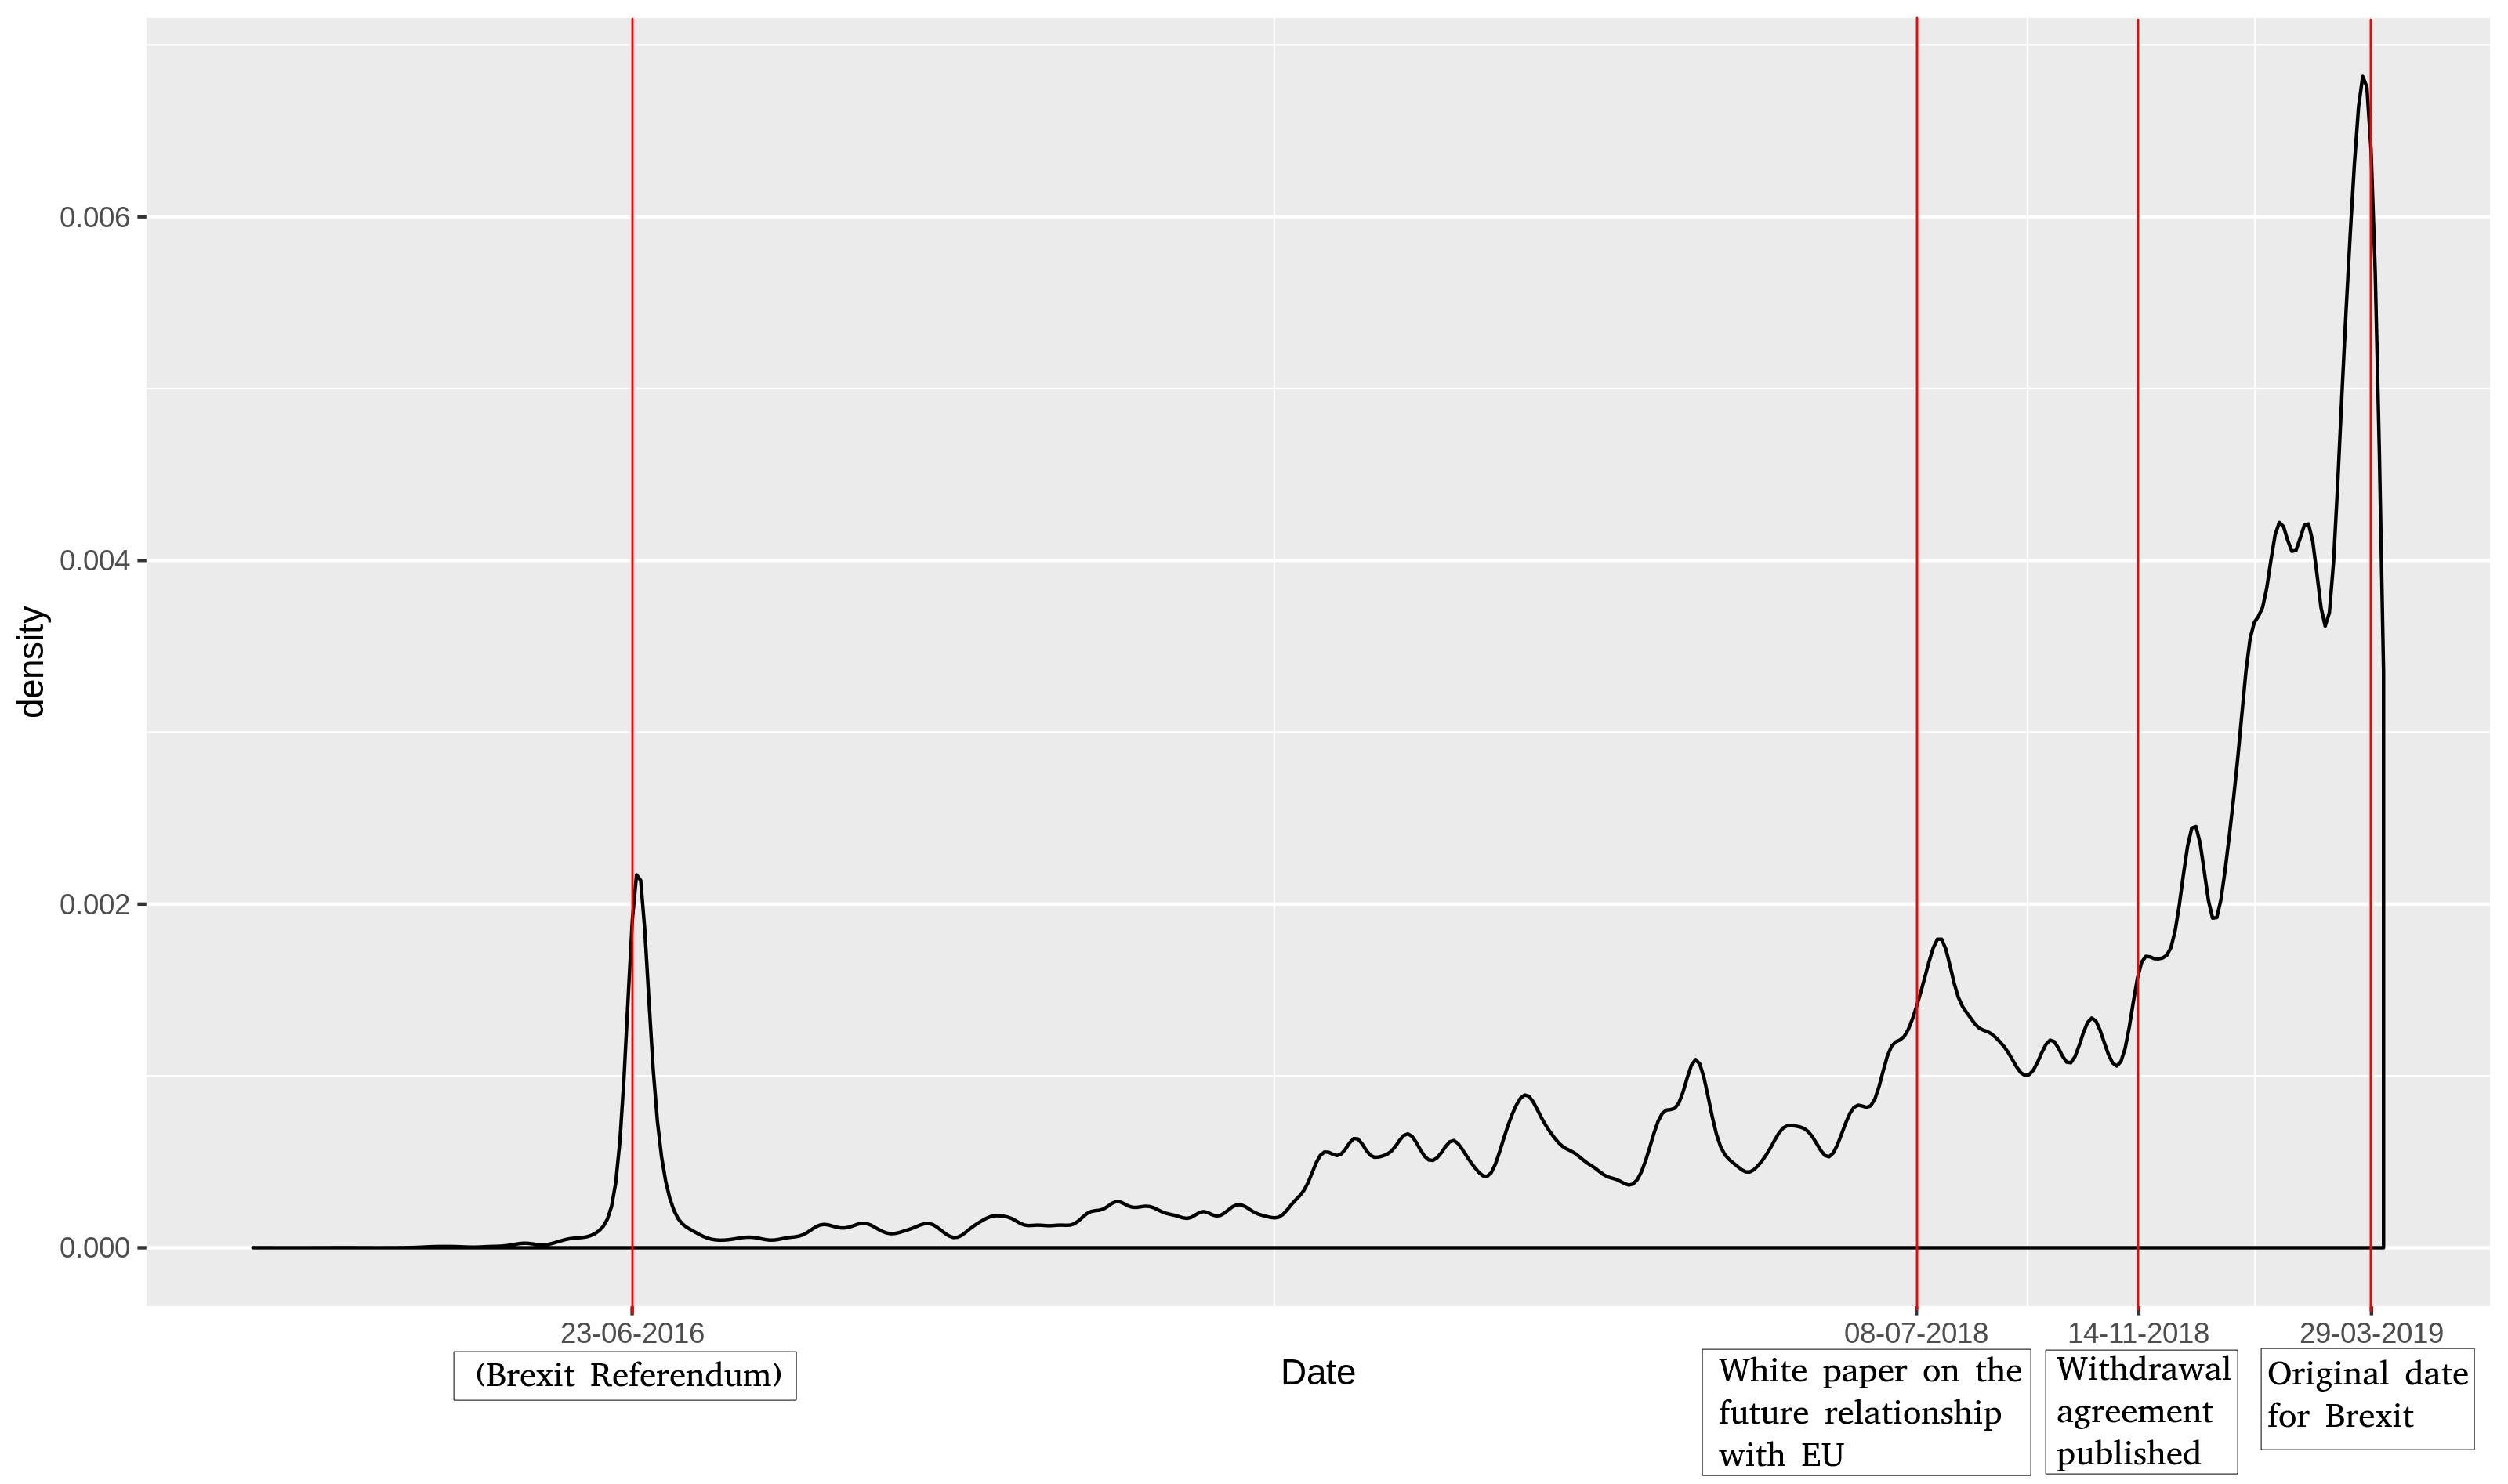
\includegraphics[height = \myheightA\textheight]{red_histo}
		\label{fig:figure_4}
	}%
	\subfloat[]{
		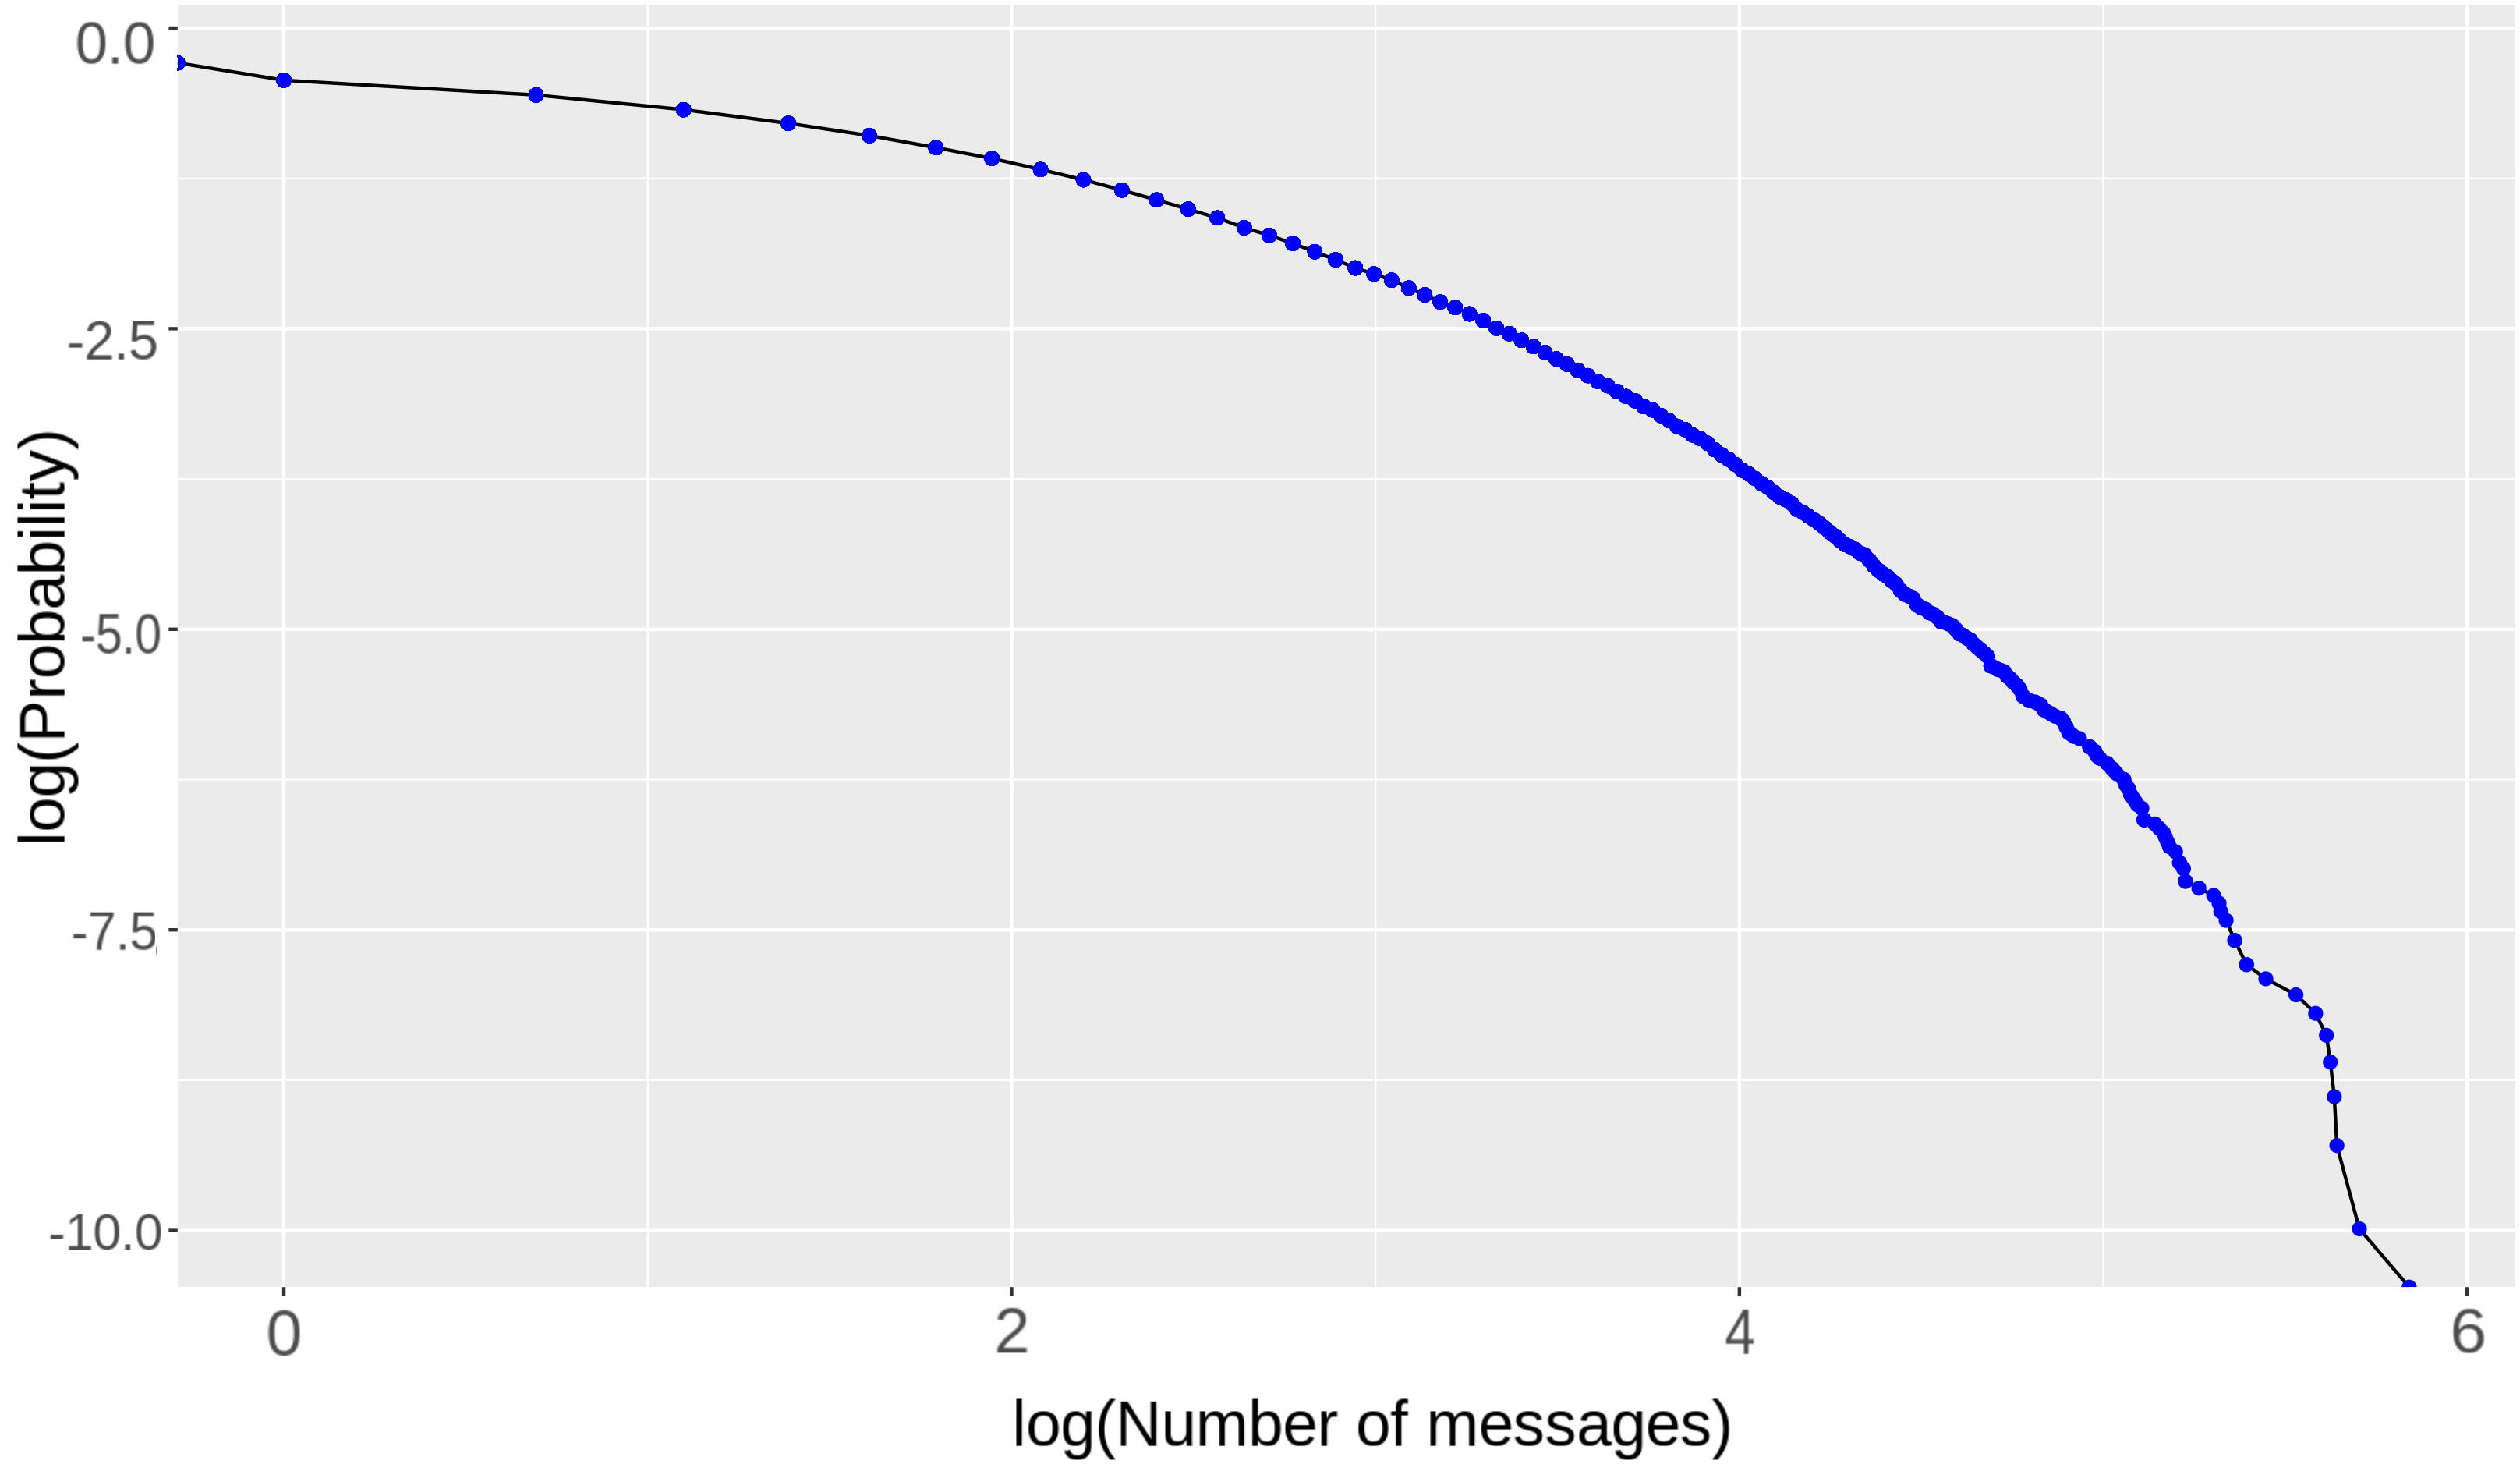
\includegraphics[height = \myheightA\textheight]{ccdf_noMess_prob}%
		\label{fig:figure_6}
	}%
	\caption{
		\textbf{(a)} Time distribution of the submissions collected from Reddit (subreddit brexit), between November, 2015 and April, 2019. 
		\textbf{(b)} Complementary Cumulative Distribution Function of the number of messages sent by each user.
	}

\end{figure}


%\textbf{Collected message distribution.} The time distribution of the collected messages is presented in Figure  \ref{fig:figure_4}. We can observe that generally there is an ascending trend, which may give a clue of the growing importance of this subject on online social platform. Even though the monotonicity is increasing, we can observe a spike in June, 2016. This is generated by the fact that on the 13th of June, 2016, British people were expected to vote for the national referendum. On the other hand, the peak in terms of number of submitted messages is in February - March 2019. This is a consequence of the official schedule of the Brexit process, which should have completed in March, 2019.

As far as the statistical structure of the submitted messages is concerned, the very vast majority of them are comments as opposed to initial thread starting messages, representing respectively 91 \% and 9 \% of the entries. Moreover, 20\% of all the unique authors are \textbf{only} thread initiators. This means they only send a single message, starting a discussion thread, in which they never post again. On the other hand, 19\% of the authors, are both thread starters and commenters, meaning that they start threads and take part actively in the discussions, posting answers in their own started thread or getting involved in other discussions. The majority of the unique users (61 \%)  are \textbf{only} commenters, meaning that they never start discussions, but usually engage in them.

Figure \ref{fig:figure_6} presents the Complementary Cumulative Distribution Function of the number of messages per user (in log log scale). It shows that a very large number of users send only a few messages, whereas there are a few users sending many messages in the observed interval. 
\hl{These users can either be opinion formers or simply paid social bots. One of the tricky tasks of this work was to identify the bots and remove them, as they do not bring new information, but most of the time reshare news and posts.}

%!TEX root = maincl.tex
%
\begin{table}[htp]
	\scriptsize
	\newcommand\mywidth{8.5cm} %% full size: 0.173
	\centering
	\caption{
		Events and time periods used for splitting the Reddit dataset.
	}
	\label{tab:time-interval-split}
%	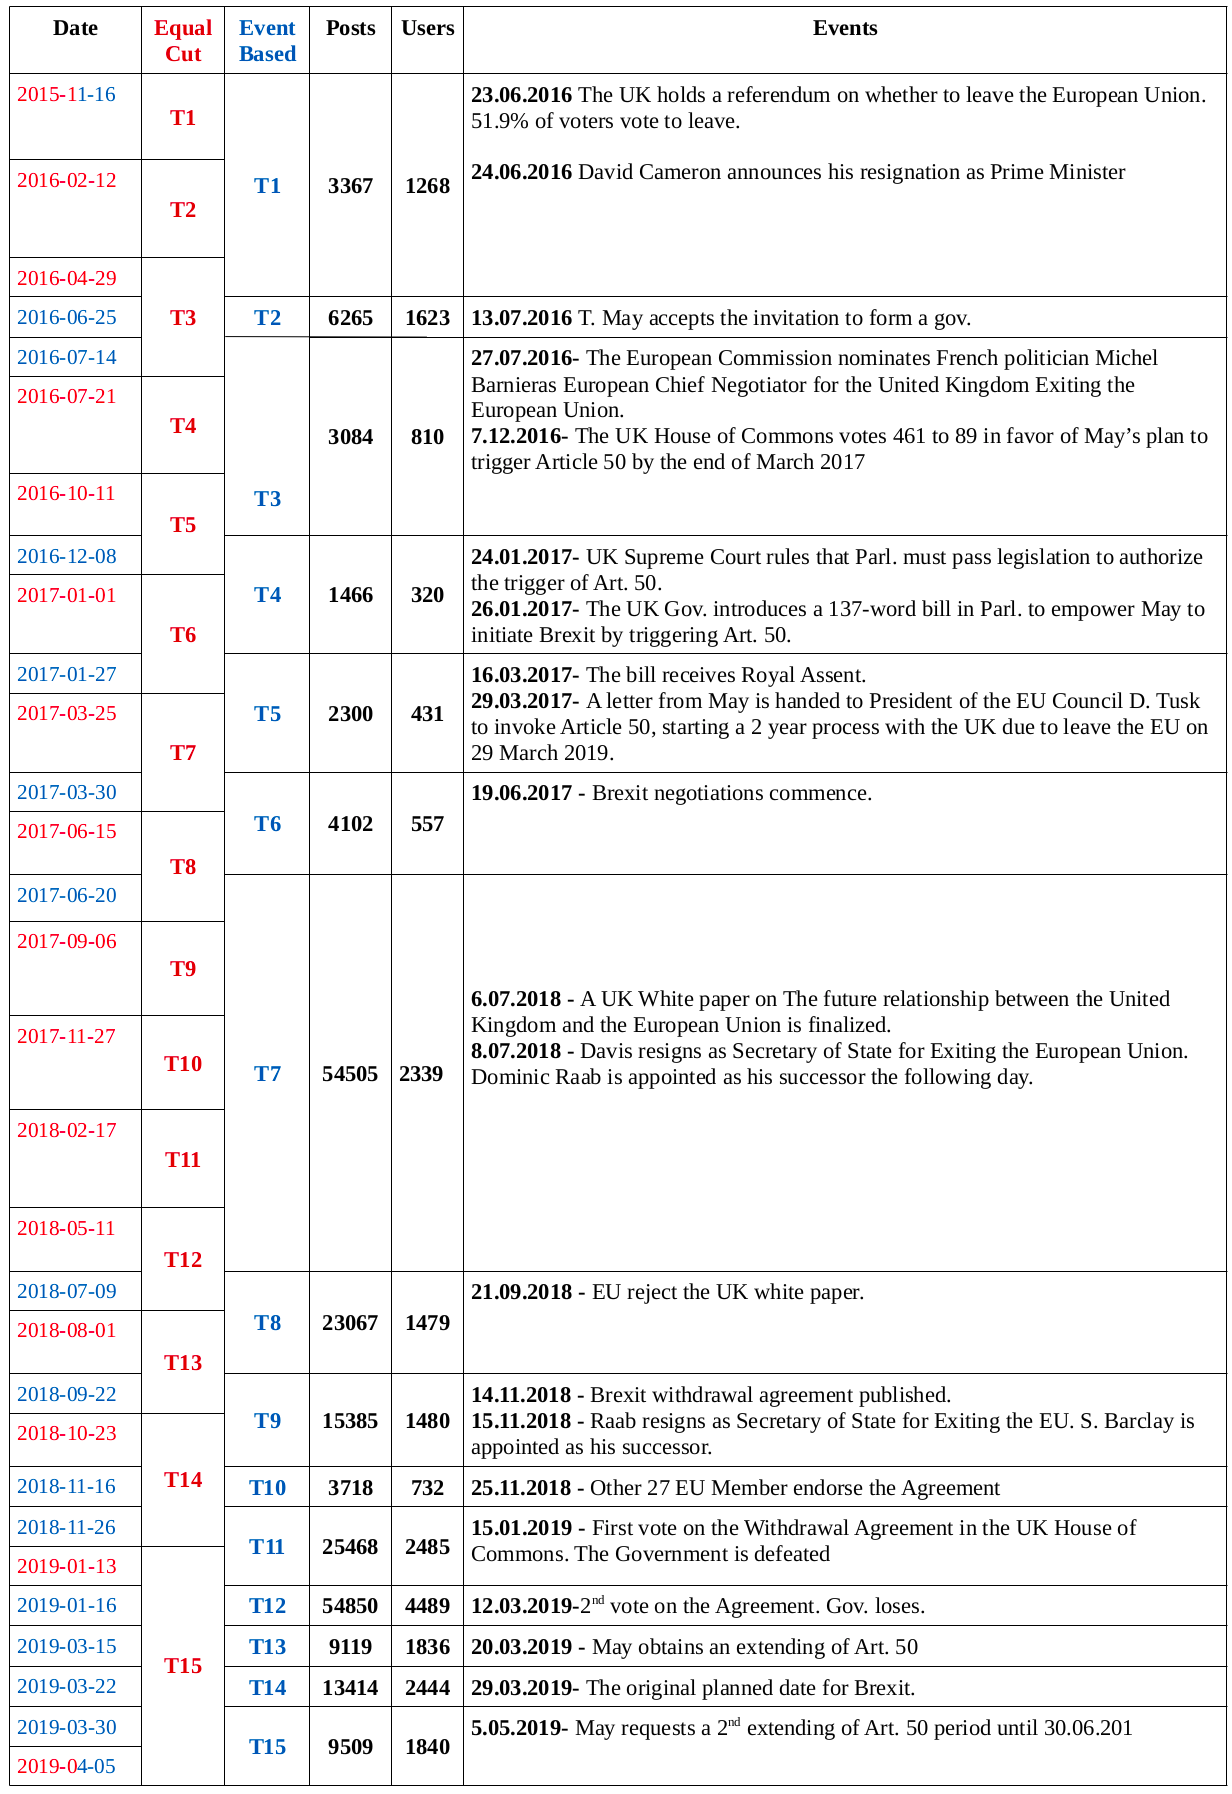
\includegraphics[width=0.93\textwidth]{per}

	\begin{tabular}{clrrp{\mywidth}}
		\toprule
		\textbf{Int.} & \multicolumn{1}{c}{\textbf{Start date}} & \multicolumn{1}{c}{\textbf{Posts}} & \multicolumn{1}{c}{\textbf{Users}} & \multicolumn{1}{c}{\textbf{Important events in the Brexit chronology}} \\ \midrule
		T1 & 2015-11-16 & 3367 & 1268 & \makecell[t{p{\mywidth}}]{
			\textbf{23 June 2016}\\
			The UK holds a referendum on whether to leave the European Union (EU). 51.9\% of voters vote to leave.\\
			\textbf{24 June 2016}\\
			David Cameron announces his resignation as Prime Minister.} \\ 
			
		T2 & 2016-06-25 & 6265 & 1623 & \makecell[t{p{\mywidth}}]{
			\textbf{13 July 2016}\\
			Theresa May accepts the Queen's invitation to form a government} \\
			
		T3 & 2016-07-14 & 3084 & 810 & \makecell[t{p{\mywidth}}]{
			\textbf{27 July 2016}\\
			The European Commission nominates French politician Michel Barnier as European Chief Negotiator for the United Kingdom Exiting the European Union.\\
			\textbf{7 December 2016}\\
			The UK House of Commons votes 461 to 89 in favour of May’s plan to trigger Article 50 by the end of March 2017} \\

		T4 & 2016-12-08 & 1466 & 320 & \makecell[t{p{\mywidth}}]{
			\textbf{24 January 2017}\\
			UK Supreme Court rules that Parl. must pass legislation to authorize the trigger of Art. 50.\\
			\textbf{26 January 2017}\\
			The UK Gov. introduces a 137-word bill in Parl. to empower May to initiate Brexit by triggering Art 50.} \\

		T5 & 2017-01-27 & 2300 & 431 & \makecell[t{p{\mywidth}}]{
			\textbf{16 March 2017}
			The bill receives Royal Assent.\\
			\textbf{29 March 2017}\\
			A letter from May is handed to President of the European Council Donald Tusk to invoke Article 50, starting a two year process with the UK due to leave the EU on 29 March 2019.} \\

		T6 & 2017-03-30 & 4102 & 557 & \makecell[t{p{\mywidth}}]{
			\textbf{19 June 2017}
			Brexit negotiations commence.} \\

		T7 & 2017-06-20 & 54505 & 2339 & \makecell[t{p{\mywidth}}]{
			\textbf{6 July 2018}\\
			A UK White paper on The future relationship between the United Kingdom and the European Union is finalized.\\
			\textbf{8 July 2018}\\
			Davis resigns as Secretary of State for Exiting the EU. Dominic Raab is appointed as his successor the following day.} \\

		T8 & 2018-07-09 & 23067 & 1479 & \makecell[t{p{\mywidth}}]{
			\textbf{21 September 2018}
			EU rejects the UK white paper.} \\

		T9 & 2018-09-22 & 15385 & 1480 & \makecell[t{p{\mywidth}}]{
			\textbf{14 November 2018}
			Brexit withdrawal agreement published.\\
			\textbf{15 November 2018}\\
			Raab resigns as Secretary of State for Exiting the EU. Stephen Barclay is appointed as his successor the following day.} \\

		T10 & 2018-11-16 & 3718 & 732 & \makecell[t{p{\mywidth}}]{
			\textbf{25 November 2018}\\
			Other 27 EU Member States endorse the Withdrawal Agreement.} \\

		T11 & 2018-11-26 & 25468 & 2485 & \makecell[t{p{\mywidth}}]{
			\textbf{15 January 2019}\\
			First meaningful vote held on the Withdrawal Agreement in the UK House of Commons. The UK Gov. is defeated by 432 votes to 202} \\

		T12 & 2019-01-16 & 54850 & 4489 & \makecell[t{p{\mywidth}}]{
			\textbf{12 March 2019}\\
			Second meaningful vote on the Withdrawal Agreement with the UK Government defeated again by 391 votes to 242.\\
			\textbf{14 March 2019}\\
			UK Gov. motion passes 412 to 202 to extend the Article 50 period.} \\

		T13 & 2019-03-15 & 9119 & 1836 & \makecell[t{p{\mywidth}}]{
			\textbf{20 March 2019}\\
			May requests the EU extend the Article 50 period until 30 June 2019.\\
			\textbf{21 March 2019}\\
			The European Council offers to extend the Article 50 period until 22 May 2019 if the Withdrawal Agreement is passed by 29 March 2019 but, if it does not, then the UK has until 12 April 2019 to indicate a way forward. The extension is formally agreed the following day.} \\
	
		T14 & 2019-03-22 & 13414 & 2444 & \makecell[t{p{\mywidth}}]{
			\textbf{29 March 2019}\\
			The original end of the Article 50 period and the original planned date for Brexit. Third vote on the Withdrawal Agreement after being separated from the Political Declaration. UK Government defeated again by 344 votes to 286.} \\
	
		T15 & 2019-03-30 & 9509 & 1840 & \makecell[t{p{\mywidth}}]{
			\textbf{5 April 2019}\\
			May requests for a second time that the EU extend the Article 50 period until 30 June 2019.} \\

		& 2019-04-05 &  &  & \textit{--dataset end--} \\ \bottomrule
	\end{tabular}

\end{table}

\section{Prediction  for Neutral}

\cl{remove paragraph ci dessous ou a verifier -> Predicting the following stance}
Furthermore, in order to explain these results, we compute volume of users corresponding to each of the 9 transitions. The results are shown in \cref{tab:volume_users}. This table explains the values from \cref{fig:table_f1_scores}. Firstly, the number of users having a Neutral - Neutral trajectory is considerably small, because of the applied filtering, namely the removal of entries having translation Neutral - Neutral which appear only once, for a given set of input features. Next, we obtain very low scores for the transitions from a pro Brexit stance to an against Brexit stance and vice-versa because the number of examples of users in these situations is very small compared to the other categories, 35 and 33 respectively. 
%!TEX root = maincl.tex
%
% Please add the following required packages to your document preamble:
% \usepackage[table,xcdraw]{xcolor}
% If you use beamer only pass "xcolor=table" option, i.e. \documentclass[xcolor=table]{beamer}
\begin{table}[htp]
	\centering
	\caption{The volume of users in the testing set for each category of transitions.}
	\label{tab:volume_users}
	\begin{tabular}{ccc}
	\toprule
	\textbf{\begin{tabular}[c]{@{}c@{}}Current\\ Stance\end{tabular}} & \textbf{\begin{tabular}[c]{@{}c@{}}Following\\ Stance\end{tabular}} & \textbf{\begin{tabular}[c]{@{}c@{}}Number of\\ Users\end{tabular}} \\ \midrule
{\color[HTML]{FE0000} Against}                                    & {\color[HTML]{FE0000} Against}                                      & 158                                                                \\ 
{\color[HTML]{FE0000} Against}                                    & {\color[HTML]{3166FF} Brexit}                                       & 33                                                                 \\ 
{\color[HTML]{FE0000} Against}                                    & {\color[HTML]{656565} Neutral}                                      & 371                                                                \\
{\color[HTML]{3166FF} Brexit}                                     & {\color[HTML]{FE0000} Against}                                      & 35                                                                 \\ 
{\color[HTML]{3166FF} Brexit}                                     & {\color[HTML]{3166FF} Brexit}                                       & 60                                                                 \\
{\color[HTML]{3166FF} Brexit}                                     & {\color[HTML]{656565} Neutral}                                      & 332                                                                \\ 
{\color[HTML]{656565} Neutral}                                    & {\color[HTML]{FE0000} Against}                                      & 387                                                                \\ 
{\color[HTML]{656565} Neutral}                                    & {\color[HTML]{3166FF} Brexit}                                       & 350                                                                \\ 
{\color[HTML]{656565} Neutral}                                    & {\color[HTML]{656565} Neutral}                                      & 27                                                                 \\ \bottomrule
\end{tabular}
\end{table}

Indeed, the chances that a user will change his position in two consecutive time-frames from totally Brexit supporting to totally against Brexit are low and this is revealed by the distribution presented in \cref{tab:volume_users}.  In most situations, there will be a transition through the intermediate Neutral state, also shown by \cref{tab:volume_users}, the number of users going from Against and Brexit to Neutral being 371 and respectively 350. This allows our classifier to understand the underlying structure of the dataset, leading to high F1-scores for these translations.

\hl{The XGBoost classifier obtains an overall F1-score of 0.57, using the FS4 feature set. We can identify two main sub-components of this score: the first one is represented by the low scores obtained when predicting transitions Brexit - Against or Brexit - Brexit, which lowers the overall score. The second sub-component is defined by the predictions involving the Neutral state, namely from Neutral to the other three states.}

Predicting the following stance a user will arrive into turns out to be a difficult task, notably when the user changes of opinion. 
\cl{verifier figure envoye par mel le 8/05 Pbl}
In \cref{fig:figure_12} we show the volume of users translating from neutral state to a Brexit supporting state or Against Brexit state, in consecutive time-frames. The left figure shows the percentage of users, while the right figure shows the exact number of users going to the two polarized states. We can observe that except the starting time-frame, where there was a strong campaign for Brexit which is reflected in the ratio of users who migrated to a Brexit stance in the second time-frame, usually the trend is in favor of the Against side. In translations from T2 to T12, neutral users tended to move to Against Brexit. However, in T12, there is a change in the trend. 

\begin{figure*}[tbp]
	\centering
	\newcommand\myheightA{0.175} %% full size: 0.173
	\subfloat[]{
		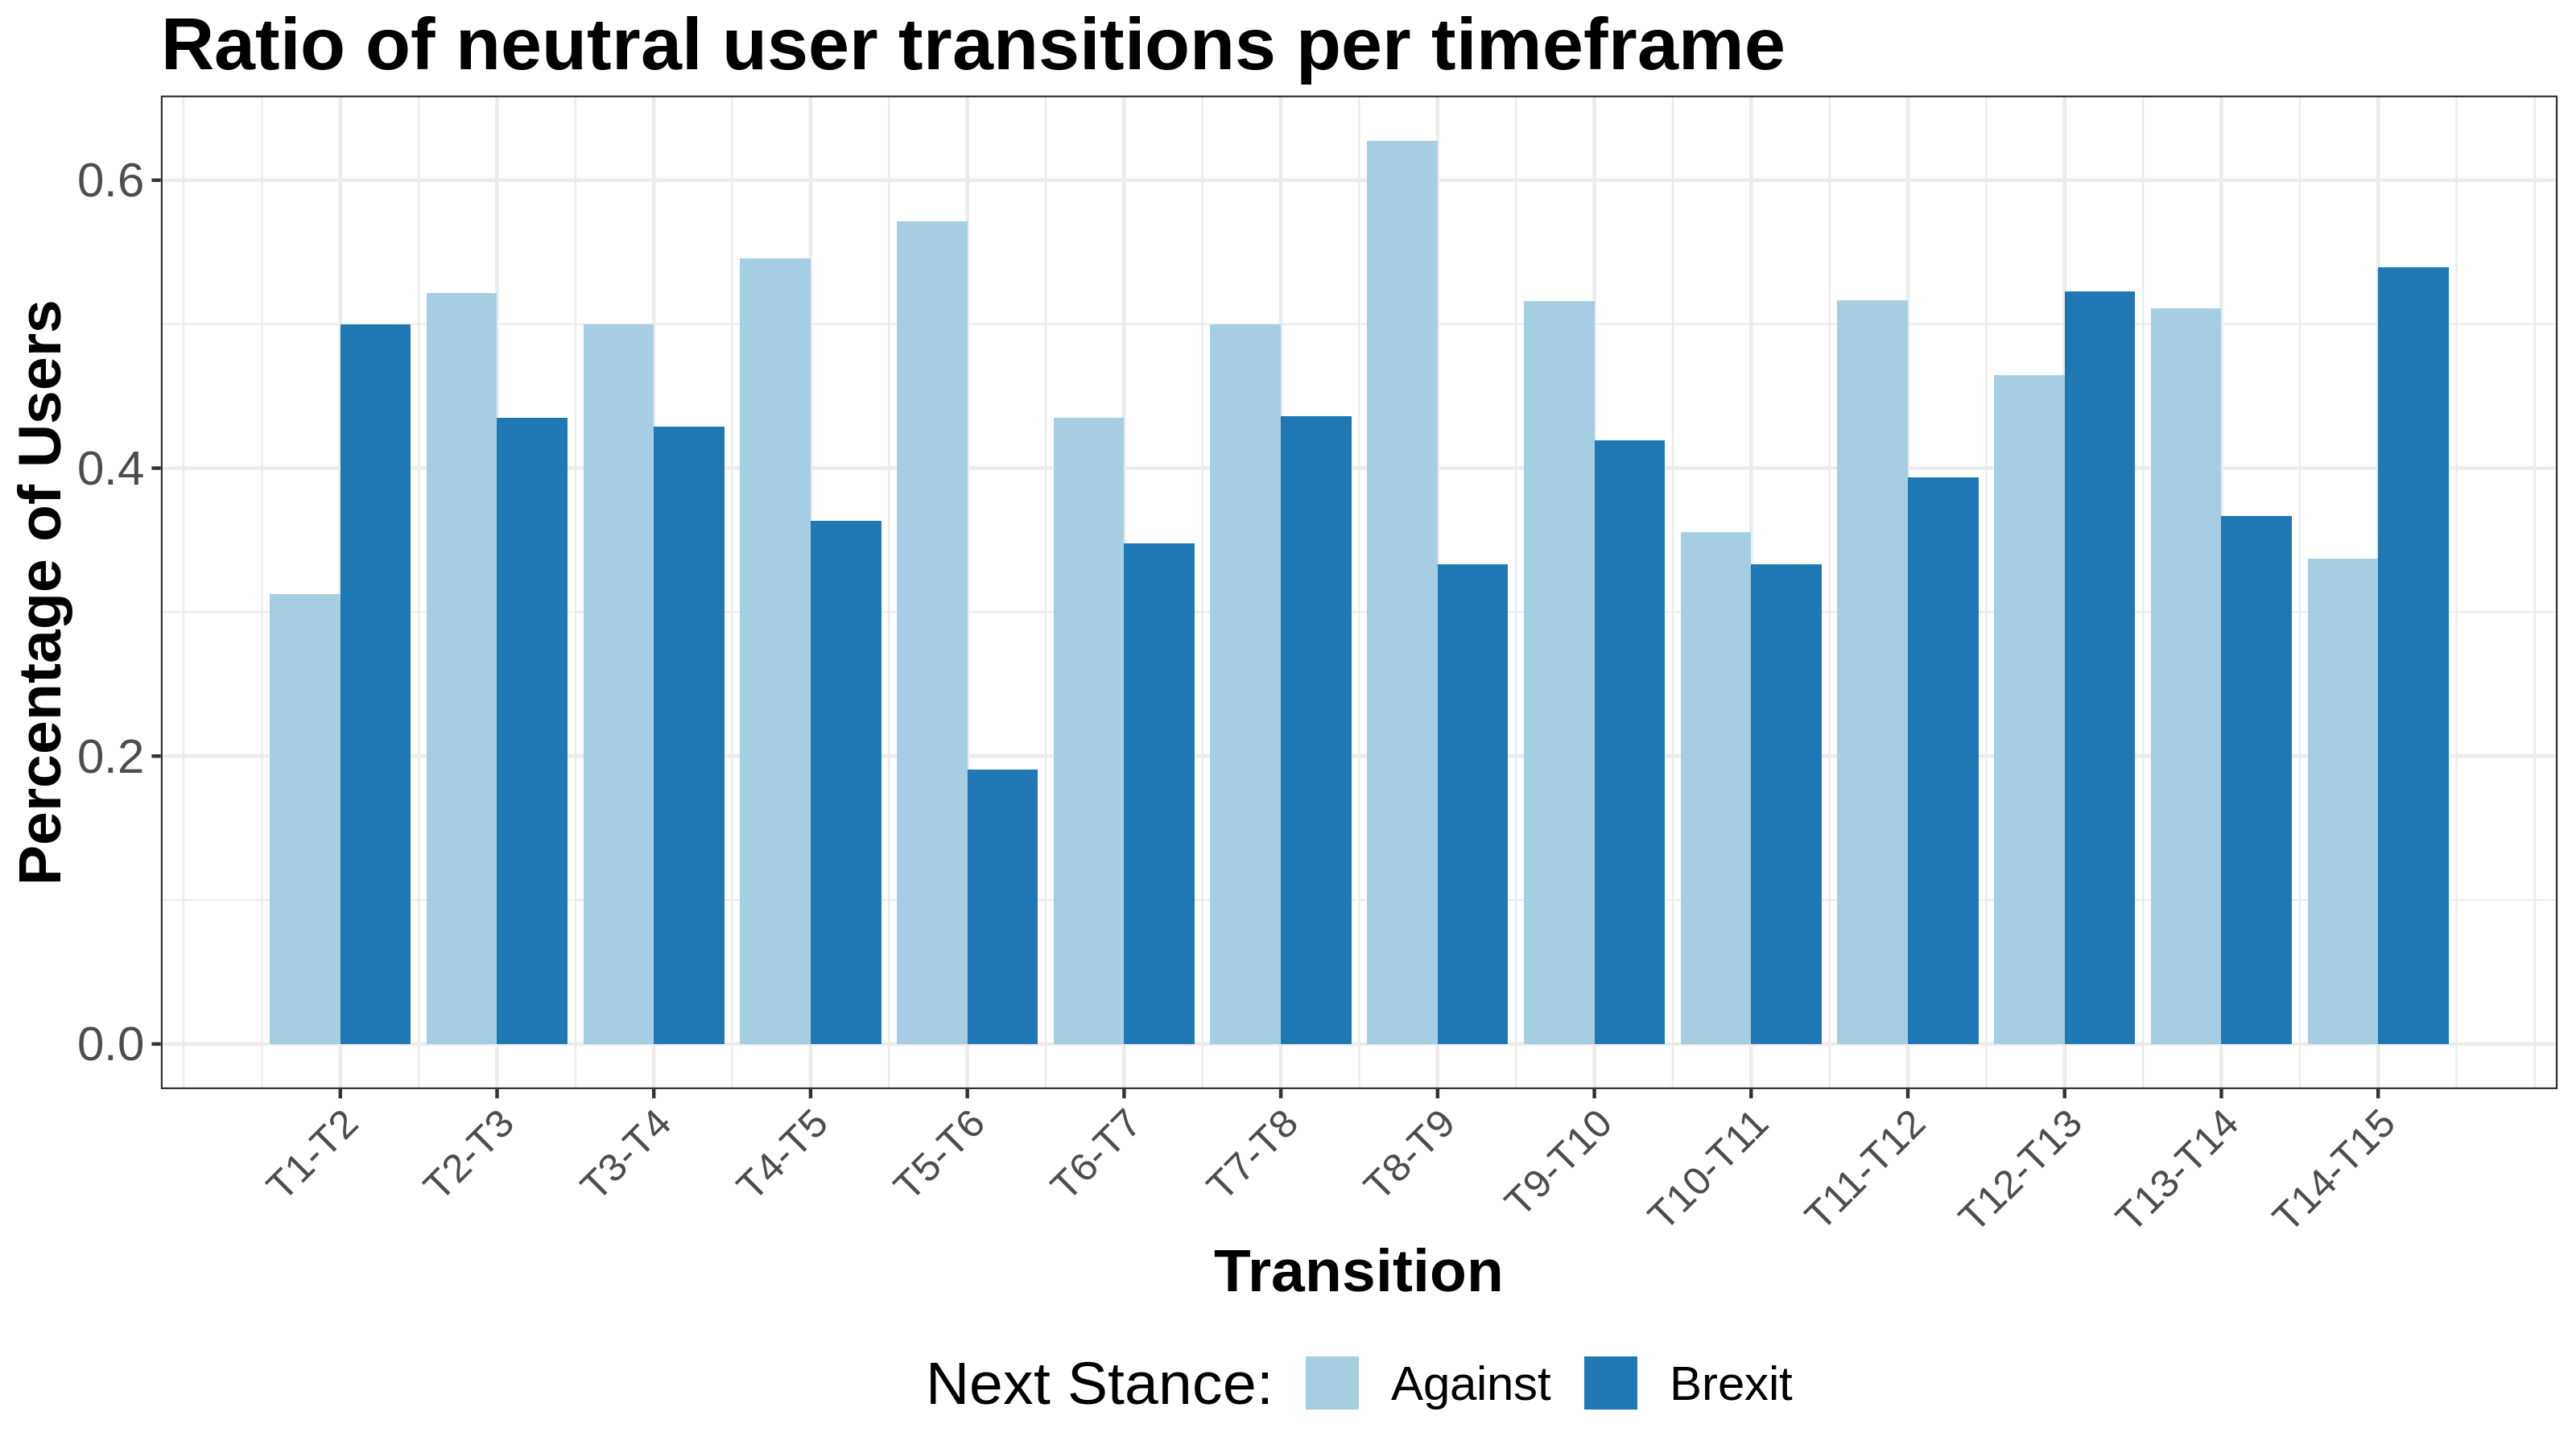
\includegraphics[height = \myheightA\textheight]{ratio_user_transitions}%
		\label{subfig:neutral-ratio}%
	}%
	\subfloat[]{
		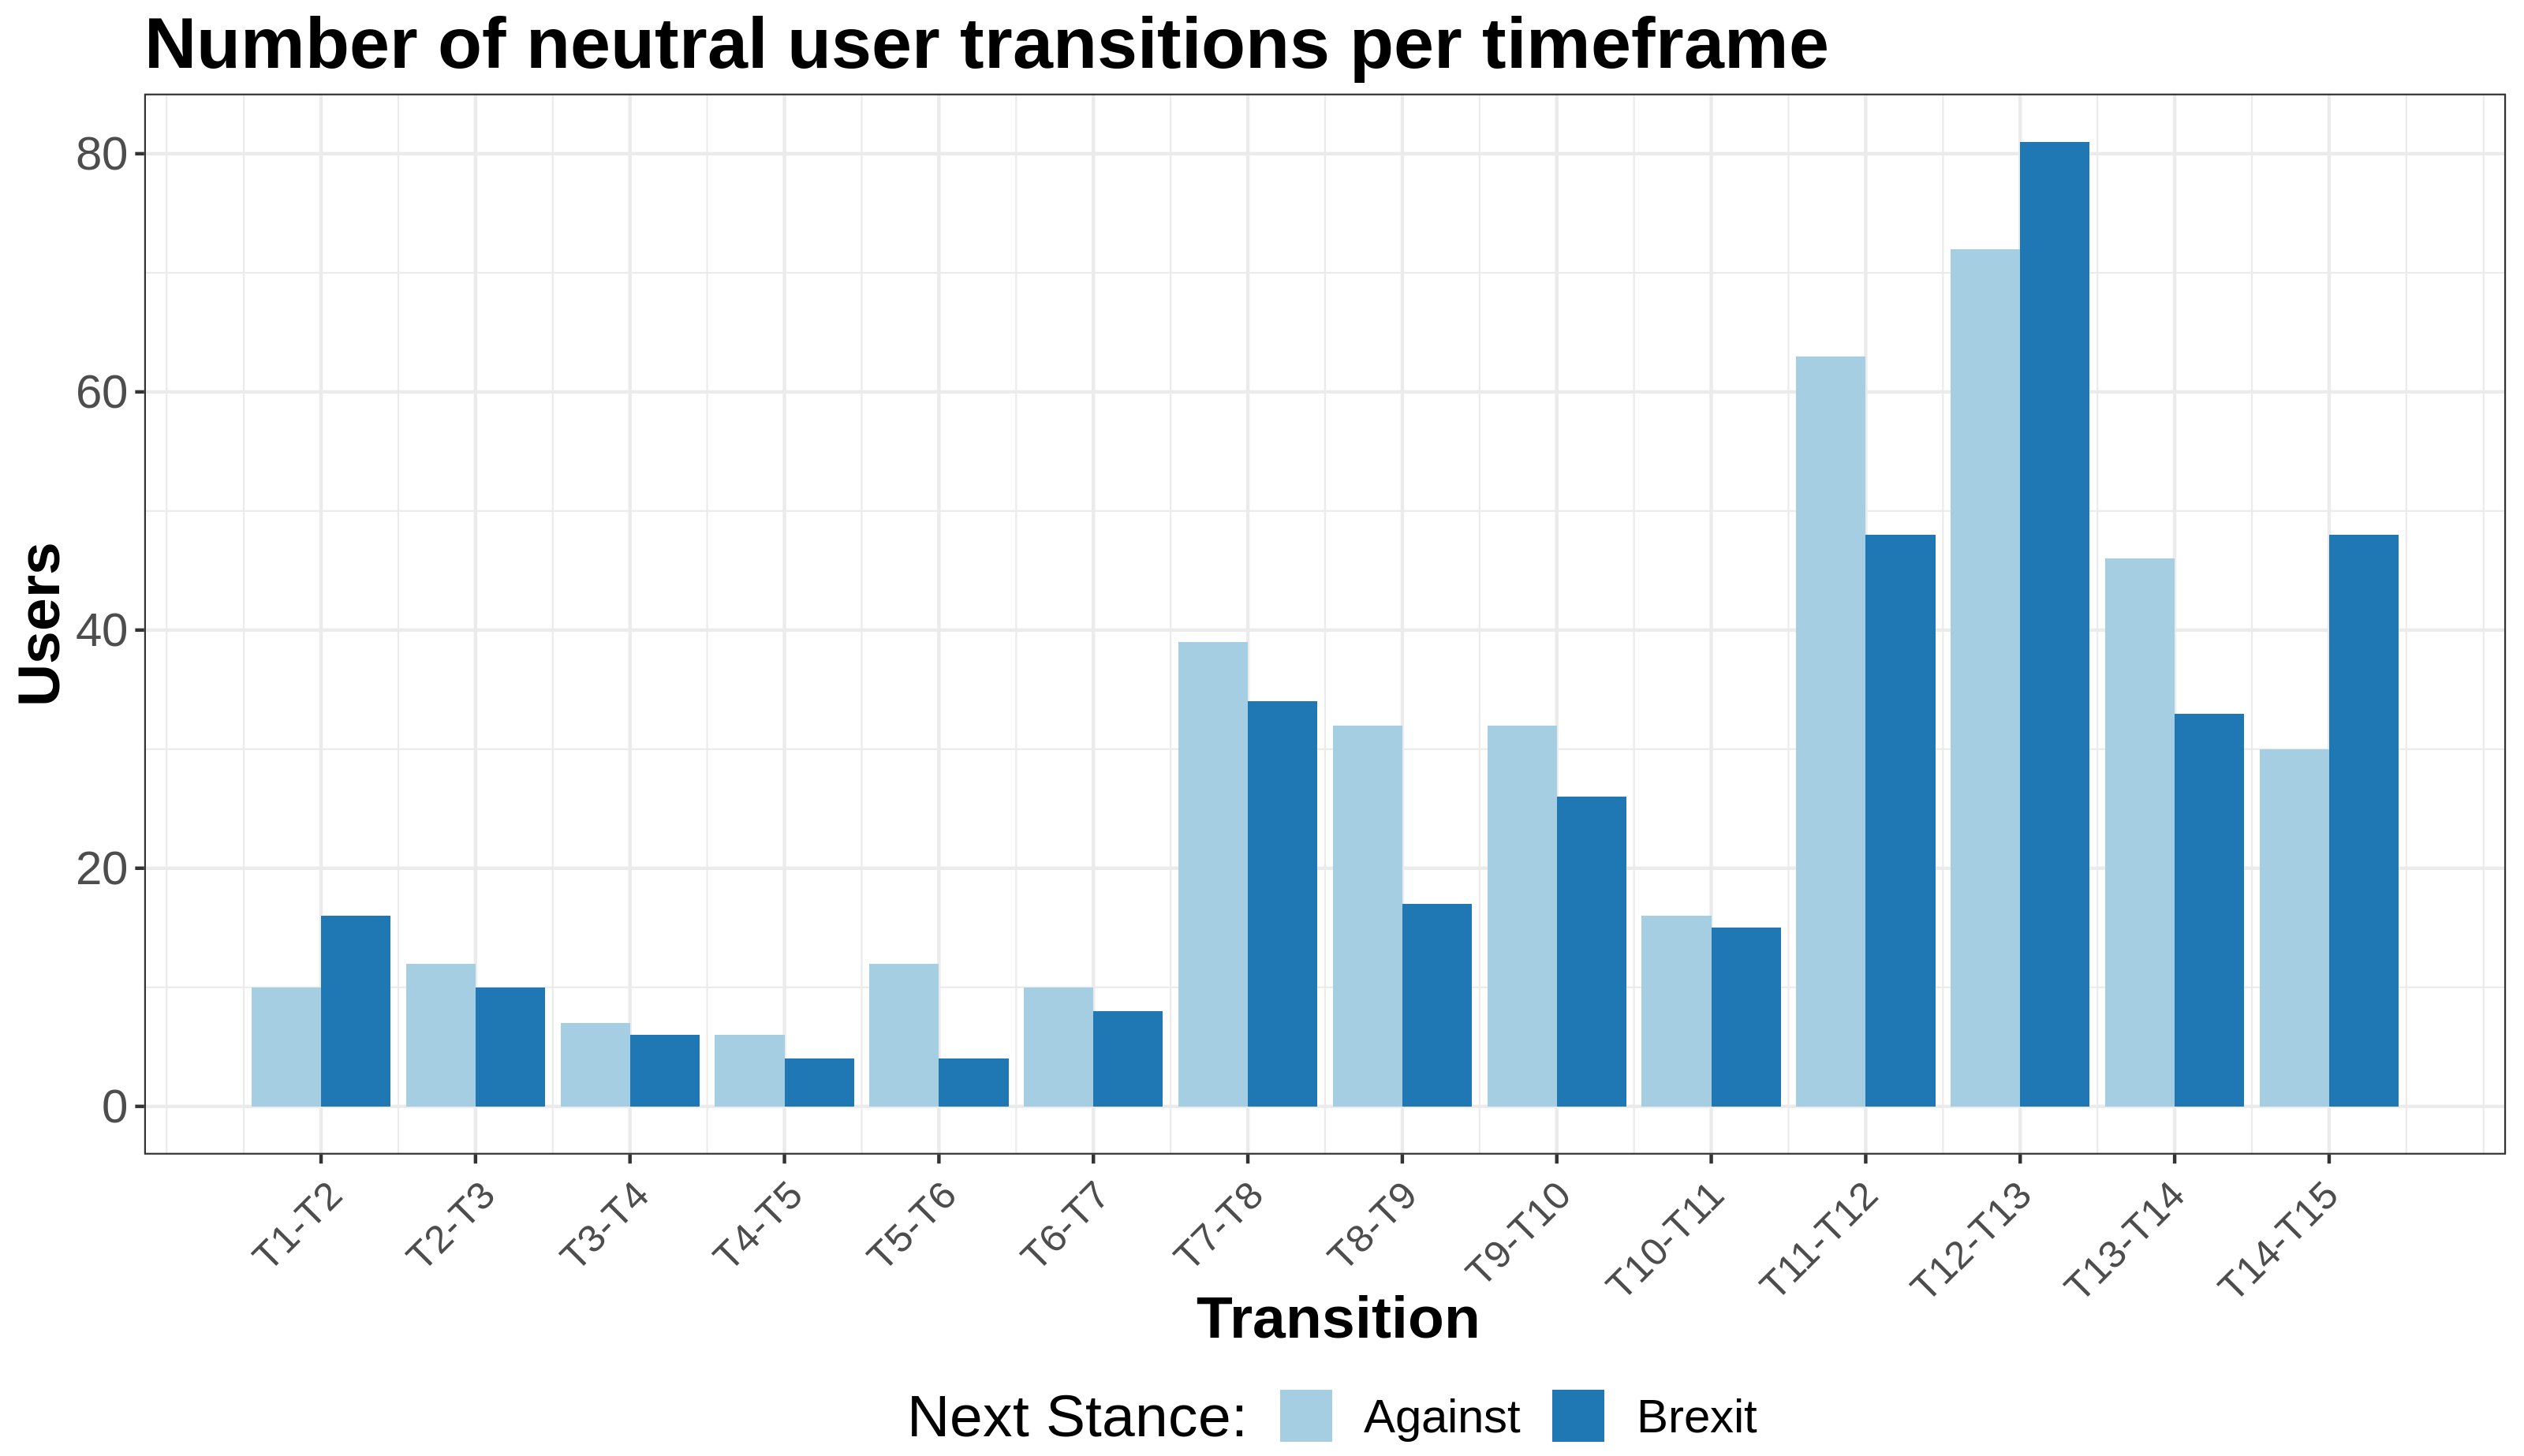
\includegraphics[height = \myheightA\textheight]{number_user_transitions}%
		\label{subfig:neutral-volume}%
	}%
	\caption{ 
		\TODO{MAR}{PDF (vectorial) version needed!}
		a) Ratio of users transitioning to the other stances in consecutive time-frames.  ratio. 
		b) Number of users transitioning to the other stances in consecutive time-frames. 
	}
	\label{fig:figure_12}
\end{figure*}

We performed some analysis on this period and found out that the main event in this period of time was the second negative vote in the Parliament for the Withdrawal Agreement negotiated by Theresa May. UK would have had to pay the European Union 39 billion pounds, which was upsetting and disappointing for people, as revealed by some of the utterances we checked (we checked utterances with high leave probability): "\textit{It's taken far too much time, we should leave hard and deal with the consequences. It will be tough for a time but there's no price not worth paying for freedom from the globalist overlords... ``It's **better** to **die free**, **than live** as a slave.'' F. Douglass}" or "\textit{Democracy? We roam the world dismantling dictatorships to install democracy, leaving failed states, but we cannot deliver the democratic will of our own population! }". We assume people tended to be disappointed by the incapability of the politicians to deliver the Brexit, thus the raise in Neutral people from time-frame 12 transitioning to Brexit in time-frame 13. 


We tested our best predictor, the XGBoost using FS4, the feature set comprising all the other sets, on users on this period of time. Thus, we considered time-frame 12 and tried to predict how many users will have a trajectory towards the Brexit side and how many will migrate towards the Against Brexit side. The results are shown in Table \ref{fig:table_story}.

%!TEX root = maincl.tex
%
\begin{table}[htp]
\centering
\caption{Number of neutral users in time-frame 12 predicted to migrate to each of the other stances in time-frame 13.
\TODO{MAR}{Bring observed volumes here, as a new line.}}
\label{fig:table_story}
\begin{tabular}{ccc}
\toprule
\textbf{Against} & \textbf{Brexit} & \textbf{Neutral} \\ \midrule
71& 83 & 4 \\ \bottomrule
\end{tabular}
\end{table}

 Even though the task of predicting the future stance of groups of users is difficult, we manged to correctly predict towards which group will neutral users migrate in a consequent period of time. This shows that our predictor correctly captured the trend and the underlying dynamics of the online population, despite the sudden change of tendancy, after a long series of similar inter-period transitions. Such kind of results can be very interesting for polling agencies trying to discover before-hand the outcome of important events debated online. What is more surprising, these results are obtained without the involvement of textual information at all in the feature sets, but just with taking advantage of the interaction between people and the diffusion of information.


\end{document}
